\documentclass[a4paper,11pt,fleqn,twoside,openright]{memoir} 	% Openright aabner kapitler paa hoejresider (openany begge)

%%%% PACKAGES %%%%

% ¤¤ Oversaettelse og tegnsaetning ¤¤ %
\usepackage[utf8]{inputenc}					% Input-indkodning af tegnsaet (UTF8)
\usepackage[english]{babel}					% Dokumentets sprog
\usepackage[T1]{fontenc}					% Output-indkodning af tegnsaet (T1)
\usepackage{ragged2e,anyfontsize}			% Justering af elementer
\usepackage{fixltx2e}						% Retter forskellige fejl i LaTeX-kernen
																			
% ¤¤ Figurer og tabeller (floats) ¤¤ %
\usepackage{graphicx} 						% Haandtering af eksterne billeder (JPG, PNG, PDF)
\usepackage{multirow}                		% Fletning af raekker og kolonner (\multicolumn og \multirow)
\usepackage{colortbl} 						% Farver i tabeller (fx \columncolor, \rowcolor og \cellcolor)
\usepackage[dvipsnames]{xcolor}				% Definer farver med \definecolor. Se mere: http://en.wikibooks.org/wiki/LaTeX/Colors
\usepackage{flafter}						% Soerger for at floats ikke optraeder i teksten foer deres reference
\let\newfloat\relax 						% Justering mellem float-pakken og memoir
\usepackage{float}							% Muliggoer eksakt placering af floats, f.eks. \begin{figure}[H]
%\usepackage{eso-pic}						% Tilfoej billedekommandoer paa hver side
%\usepackage{wrapfig}						% Indsaettelse af figurer omsvoebt af tekst. \begin{wrapfigure}{Placering}{Stoerrelse}
%\usepackage{multicol}         	        	% Muliggoer tekst i spalter
%\usepackage{rotating}						% Rotation af tekst med \begin{sideways}...\end{sideways}
\usepackage{array}


% ¤¤ Matematik mm. ¤¤
\usepackage{amsmath,amssymb,stmaryrd} 		% Avancerede matematik-udvidelser
\usepackage{mathtools}						% Andre matematik- og tegnudvidelser
\usepackage{textcomp}                 		% Symbol-udvidelser (f.eks. promille-tegn med \textperthousand )
\usepackage{siunitx}						% Flot og konsistent praesentation af tal og enheder med \si{enhed} og \SI{tal}{enhed}
\sisetup{output-decimal-marker = {,}}		% Opsaetning af \SI (DE for komma som decimalseparator) 
\usepackage[version=3]{mhchem} 				% Kemi-pakke til flot og let notation af formler, f.eks. \ce{Fe2O3}
%\usepackage{rsphrase}						% Kemi-pakke til RS-saetninger, f.eks. \rsphrase{R1}

% ¤¤ Referencer og kilder ¤¤ %
\usepackage[danish]{varioref}				% Muliggoer bl.a. krydshenvisninger med sidetal (\vref)
\usepackage{natbib}							% Udvidelse med naturvidenskabelige citationsmodeller
%\usepackage{xr}							% Referencer til eksternt dokument med \externaldocument{<NAVN>}
%\usepackage{glossaries}					% Terminologi- eller symbolliste (se mere i Daleifs Latex-bog)

% Quotation %
\usepackage{csquotes}

% ¤¤ Misc. ¤¤ %
\usepackage{listings}						% Placer kildekode i dokumentet med \begin{lstlisting}...\end{lstlisting}
\usepackage{lipsum}							% Dummy text \lipsum[..]
\usepackage[shortlabels]{enumitem}			% Muliggoer enkelt konfiguration af lister
\usepackage{pdfpages}						% Goer det muligt at inkludere pdf-dokumenter med kommandoen \includepdf[pages={x-y}]{fil.pdf}	
\pdfoptionpdfminorversion=6					% Muliggoer inkludering af pdf dokumenter, af version 1.6 og hoejere
\pretolerance=2500 							% Justering af afstand mellem ord (hoejt tal, mindre orddeling og mere luft mellem ord)

% Kommentarer og rettelser med \fxnote. Med 'final' i stedet for 'draft' udloeser hver note en error i den faerdige rapport.
\usepackage[footnote,draft,danish,silent,nomargin]{fixme}		

\usepackage{todonotes}

\usepackage{lastpage}

%%%% CUSTOM SETTINGS %%%%

% ¤¤ Marginer ¤¤ %
\setlrmarginsandblock{3.5cm}{2.5cm}{*}		% \setlrmarginsandblock{Indbinding}{Kant}{Ratio}
\setulmarginsandblock{2.5cm}{3.0cm}{*}		% \setulmarginsandblock{Top}{Bund}{Ratio}
\checkandfixthelayout 						% Oversaetter vaerdier til brug for andre pakker

%	¤¤ Afsnitsformatering ¤¤ %
\setlength{\parindent}{0mm}           		% Stoerrelse af indryk
\setlength{\parskip}{3mm}          			% Afstand mellem afsnit ved brug af double Enter
\linespread{1,1}							% Linie afstand

%Definition bokses %
\usepackage{xcolor}
\usepackage{ntheorem}
\usepackage{mdframed}

\theoremstyle{break}
\theoremheaderfont{\bfseries}
\newmdtheoremenv[%
linecolor=gray,leftmargin=60,%
rightmargin=40,
backgroundcolor=gray!40,%
innertopmargin=8pt,%
ntheorem]{defi}{Definition}[section]

% ¤¤ Litteraturlisten ¤¤ %
\bibpunct[,]{[}{]}{;}{a}{,}{,} 				% Definerer de 6 parametre ved Harvard henvisning (bl.a. parantestype og seperatortegn)
\bibliographystyle{bibtex/harvard}			% Udseende af litteraturlisten.

% ¤¤ Indholdsfortegnelse ¤¤ %
\setsecnumdepth{subsection}		 			% Dybden af nummerede overkrifter (part/chapter/section/subsection)
\maxsecnumdepth{subsection}					% Dokumentklassens graense for nummereringsdybde
\settocdepth{subsection} 					% Dybden af indholdsfortegnelsen

% ¤¤ Lister ¤¤ %
\setlist{
  topsep=0pt,								% Vertikal afstand mellem tekst og listen
  itemsep=-1ex,								% Vertikal afstand mellem items
} 

% ¤¤ Visuelle referencer ¤¤ %
\usepackage[colorlinks]{hyperref}			% Danner klikbare referencer (hyperlinks) i dokumentet.
\hypersetup{colorlinks = true,				% Opsaetning af farvede hyperlinks (interne links, citeringer og URL)
    linkcolor = black,
    citecolor = black,
    urlcolor = black
}

% ¤¤ Opsaetning af figur- og tabeltekst ¤¤ %
\captionnamefont{\small\bfseries\itshape}	% Opsaetning af tekstdelen ('Figur' eller 'Tabel')
\captiontitlefont{\small}					% Opsaetning af nummerering
\captiondelim{. }							% Seperator mellem nummerering og figurtekst
\hangcaption								% Venstrejusterer flere-liniers figurtekst under hinanden
\captionwidth{\linewidth}					% Bredden af figurteksten
\setlength{\belowcaptionskip}{0pt}			% Afstand under figurteksten
		
% ¤¤ Opsaetning af listings ¤¤ %
\definecolor{commentGreen}{RGB}{34,139,24}
\definecolor{stringPurple}{RGB}{208,76,239}

\lstset{
  numbers=left,
  stepnumber=1,    
  firstnumber=1,
  numberfirstline=true
}

\usepackage{xcolor}

\lstdefinestyle{MyLang}{
    basicstyle=\small\ttfamily\color{magenta},%
    breaklines=true,%                                      allow line breaks
    moredelim=[s][\color{green!50!black}\ttfamily]{'}{'},% single quotes in green
    moredelim=*[s][\color{black}\ttfamily]{options}{\}},%  options in black (until trailing })
    commentstyle={\color{gray}\itshape},%                  gray italics for comments
    morecomment=[l]{//},%                                  define // comment
    emph={%
        %                                            literal strings listed here
        },emphstyle={\color{blue}\ttfamily},%              and formatted in blue
    alsoletter={:,|,;},%
    morekeywords={:,|,;},%                                 define the special characters
    keywordstyle={\color{black}},%                         and format them in black  
}	
\lstset{language=Matlab,					% Sprog
	basicstyle=\ttfamily\scriptsize,		% Opsaetning af teksten
	%keywords={for,if,while,else,elseif,		% Noegleord at fremhaeve
	%		  end,break,return,case,
	%		  switch,function},
	keywordstyle=\color{blue},				% Opsaetning af noegleord
	commentstyle=\color{commentGreen},		% Opsaetning af kommentarer
	stringstyle=\color{stringPurple},		% Opsaetning af strenge
	showstringspaces=false,					% Mellemrum i strenge enten vist eller blanke
	%numbers=left, numberstyle=\tiny,		% Linjenumre
	extendedchars=true, 					% Tillader specielle karakterer
	columns=flexible,						% Kolonnejustering
	breaklines, breakatwhitespace=true,		% Bryd lange linjer
}



% ¤¤ Navngivning ¤¤ %
%\addto\captionsdanish{
%	\renewcommand\appendixname{Appendiks}
%	\renewcommand\contentsname{Indholdsfortegnelse}	
%	\renewcommand\appendixpagename{Appendiks}
%	\renewcommand\appendixtocname{Appendiks}
%	\renewcommand\cftchaptername{\chaptername~}				% Skriver "Kapitel" foran kapitlerne i indholdsfortegnelsen
%	\renewcommand\cftappendixname{\appendixname~}			% Skriver "Appendiks" foran appendiks i indholdsfortegnelsen
%	}

% ¤¤ Kapiteludssende ¤¤ %
\definecolor{numbercolor}{gray}{0.7}		% Definerer en farve til brug til kapiteludseende
\newif\ifchapternonum

\makechapterstyle{jenor}{					% Definerer kapiteludseende frem til ...
  \renewcommand\beforechapskip{0pt}
  \renewcommand\printchaptername{}
  \renewcommand\printchapternum{}
  \renewcommand\printchapternonum{\chapternonumtrue}
  \renewcommand\chaptitlefont{\fontfamily{pbk}\fontseries{db}\fontshape{n}\fontsize{25}{35}\selectfont\raggedleft}
  \renewcommand\chapnumfont{\fontfamily{pbk}\fontseries{m}\fontshape{n}\fontsize{1in}{0in}\selectfont\color{numbercolor}}
  \renewcommand\printchaptertitle[1]{%
    \noindent
    \ifchapternonum
    \begin{tabularx}{\textwidth}{X}
    {\let\\\newline\chaptitlefont ##1\par} 
    \end{tabularx}
    \par\vskip-2.5mm\hrule
    \else
    \begin{tabularx}{\textwidth}{Xl}
    {\parbox[b]{\linewidth}{\chaptitlefont ##1}} & \raisebox{-15pt}{\chapnumfont \thechapter}
    \end{tabularx}
    \par\vskip2mm\hrule
    \fi
  }
}											% ... her

\chapterstyle{jenor}						% Valg af kapiteludseende - Google 'memoir chapter styles' for alternativer

% ¤¤ Sidehoved ¤¤ %

\makepagestyle{Uni}							% Definerer sidehoved og sidefod udseende frem til ...
\makepsmarks{Uni}{%
	\createmark{chapter}{left}{shownumber}{}{. \ }
	\createmark{section}{right}{shownumber}{}{. \ }
	\createplainmark{toc}{both}{\contentsname}
	\createplainmark{lof}{both}{\listfigurename}
	\createplainmark{lot}{both}{\listtablename}
	\createplainmark{bib}{both}{\bibname}
	\createplainmark{index}{both}{\indexname}
	\createplainmark{glossary}{both}{\glossaryname}
}
\nouppercaseheads											% Ingen Caps oenskes

\makeevenhead{Uni}{Group SW408F16}{}{\leftmark}				% Definerer lige siders sidehoved (\makeevenhead{Navn}{Venstre}{Center}{Hoejre})
\makeoddhead{Uni}{\rightmark}{}{Aalborg University}			% Definerer ulige siders sidehoved (\makeoddhead{Navn}{Venstre}{Center}{Hoejre})
\makeevenfoot{Uni}{\thepage}{}{}							% Definerer lige siders sidefod (\makeevenfoot{Navn}{Venstre}{Center}{Hoejre})
\makeoddfoot{Uni}{}{}{\thepage}								% Definerer ulige siders sidefod (\makeoddfoot{Navn}{Venstre}{Center}{Hoejre})
\makeheadrule{Uni}{\textwidth}{0.5pt}						% Tilfoejer en streg under sidehovedets indhold
\makefootrule{Uni}{\textwidth}{0.5pt}{1mm}					% Tilfoejer en streg under sidefodens indhold

\copypagestyle{Unichap}{Uni}								% Sidehoved for kapitelsider defineres som standardsider, men med blank sidehoved
\makeoddhead{Unichap}{}{}{}
\makeevenhead{Unichap}{}{}{}
\makeheadrule{Unichap}{\textwidth}{0pt}
\aliaspagestyle{chapter}{Unichap}							% Den ny style vaelges til at gaelde for chapters
															% ... her
															
\pagestyle{Uni}												% Valg af sidehoved og sidefod (benyt "plain" for ingen sidehoved/fod)


%%%% CUSTOM COMMANDS %%%%

% ¤¤ Billede hack ¤¤ %										% Indsaet figurer nemt med \figur{Stoerrelse}{Fil}{Figurtekst}{Label}
\newcommand{\figur}[4]{
		\begin{figure}[H] \centering
			\includegraphics[width=#1\textwidth]{billeder/#2}
			\caption{#3}\label{#4}
		\end{figure} 
}

\newcommand\tab[1][1cm]{\hspace*{#1}}

% ¤¤ Specielle tegn ¤¤ %
\newcommand{\decC}{^{\circ}\text{C}}
\newcommand{\dec}{^{\circ}}
\newcommand{\m}{\cdot}


%%%% ORDDELING %%%%

\hyphenation{}											% Preamble indlaeses
\raggedbottom													% Soerger for at LaTeX ikke "straekker" teksten

%\includeonly{file1,file2}										% Inkluder kun specifikke filer (kommasepareret liste)

\begin{document}												% Starter dokumentet - obligatorisk


\frontmatter													% Forindhold - nummereres med romertal

	\thispagestyle{empty}
\begin{flushright}
\vspace{3cm}

\phantom{hul}

\phantom{hul}

\phantom{hul}

\textsl{\Huge Dumpsty} \\ \vspace{1cm}

\rule{13cm}{3mm} \\ \vspace{1.5cm}
\vspace{1cm}

%\includegraphics[width=0.9\textwidth]{}


\vspace{7cm} 
\textsc{\Large P5 Project \\
Group SW510E16 \\
Software\\
Aalborg University\\
21st Dec 2016\\}
\end{flushright}

\cleardoublepage												% Indsaetter tom side, saa naeste kapitel starter paa hoejre side (hvis noedvendigt)
% Dette er LaTeX-versionen af titelbladet for TNB studenterrapporter
% Filen kræver:
% Universitetets logo:  AAU-logo-stud-UK eller AAU-logo-stud-DK
% Synopsis: En fil ved navn synopsis.tex

% Udarbejdet af: Jesper Nørgaard (jesper@noergaard.eu) 10. april 2012

\phantomsection
\pdfbookmark[0]{Titelblad}{titelblad}
\thispagestyle{empty}

\begin{minipage}[t]{0.48\textwidth}
\vspace*{-25pt}			%\vspace*{-9pt}

\includegraphics[height=4cm]{billeder/AAU-logo-stud-UK-RGB}
\end{minipage}
\hfill
\begin{minipage}[t]{0.48\textwidth}
{\small 
\textbf{Fourth semester at}\\
\textbf{Department of Computer Science}  \\
Software \\
Selma Lagerlöfs Vej 300 \\
9220 Aalborg East, DK \\
http://www.cs.aau.dk/}
\end{minipage}

\vspace*{1cm}

\begin{minipage}[t]{0.48\textwidth}
\textbf{Title:} \\[5pt]\bigskip\hspace{2ex}
Dumpsty

\textbf{Project:} \\[5pt]\bigskip\hspace{2ex}
P5-project

\textbf{Project period:} \\[5pt]\bigskip\hspace{2ex}
September 2016 - December 2016

\textbf{Project group:} \\[5pt]\bigskip\hspace{2ex}
SW510E16	

\textbf{Participants:} \\[5pt]\hspace*{2ex}
Christian Dannesboe \\\hspace*{2ex}
Frederik Børsting Lund \\\hspace*{2ex}
Karrar Al-Sami \\\hspace*{2ex}
Mark Kloch Haurum \\\hspace*{2ex}
Lasse Lyngø Nielsen \\\hspace*{2ex}
Søren Lyng \\\hspace*{2ex}

\textbf{Supervisor:} \\[5pt]\hspace*{2ex}
Bent Thomsen

\vspace*{1cm}


\textbf{Pagecount: \pageref{LastPage}} \\
\textbf{Appendix range: 26} \\ 
\textbf{Published 21-12-2016}

\end{minipage}
\hfill
\begin{minipage}[t]{0.483\textwidth}
Synopsis: \\[5pt]
\fbox{\parbox{7cm}{\bigskipThis project is about the design and implementation of a trash bin which is to catch the trash thrown at it. This is done using a Arduino Mega 2560 for the trash bin and a Microsoft Kinect for detecting and tracking the thrown trash. 
\newline

The report covers the analysis of the problem and hardware, a design specification, system design and implementation. The system is then tested and the results are discussed and concluded upon. 
\newline



\bigskip}}
\end{minipage}

\vfill

{\footnotesize\itshape The content of the article is freely available, but may only be published with reference to the article.}

% Rapportens indhold er frit tilgængeligt, men offentliggørelse (med kildeangivelse) må kun ske efter aftale med forfatterne.
% The content of the report is freely available, but publication (with source reference) may only take place in agreement with the authors.

\cleardoublepage
\chapter*{Preface}
This report is part of the fifth semester project made by project group SW510E16 at Aalborg University, Software Engineering starting from the 2nd of September to the 21st of December 2016. \newline
The project is based on the \textit{Aalborg-model} study method, where problem and project based learning is the focus. The theme of this semester is to make an embedded system with real-time constraints. The project group chose to make a trash bin that should be able to catch the trash thrown at it. \newline

The project group would like to thank the project supervisor Bent Thomsen, for his  support and help throughout the project. 
\newline
\newline
\newline
\newline


{\Huge\textbf{Signatures}}
\newline
\newline


\begin{table}[H]
	\centering
	\begin{tabular}{c c c}
		\underline{\phantom{mmmmmmmmmmmmmm}} & \underline{\phantom{mmmmmmmmmmmmmm}} & \underline{\phantom{mmmmmmmmmmmmmm}} \\
		Christian Dannesboe			& Frederik Børsting Lund 		& Karrar Al-Sami 			\\
		&&\\
		&&\\
		\underline{\phantom{mmmmmmmmmmmmmm}} & \underline{\phantom{mmmmmmmmmmmmmm}} & \underline{\phantom{mmmmmmmmmmmmmm}} \\
		Mark Kloch Haurum			& Lasse Lyngø Nielsen 		& Søren Lyng 				\\
		&&\\
		&&\\
		
	\end{tabular}
\end{table}


\chapter*{Reading guide}
Throughout the report sources are referred to by the Harvard citation method. When a source is listed in the report, the last name of the author and a publication year is listed. The sources are all listed alphabetically in the \textit{\textbf{Bibliography}} chapter. \newline
\textit{This is an example of a source listed in the report: \textbf{\citep{safe}}.} \newline
The source may refer to either the whole section or to only that sentence. The way this differs depends on the placement of the dot. If the dot is after the source, then that source refers to the sentence and if the dot is before the source, then the source refers to the whole section. 


When referring to figures, tables and source code, numbers are used. Depending on which chapter and number of figure/table, the number is defined. \newline
\textit{This example can be used: In chapter X we want to refer to the second figure. This is done by giving the figure number \textbf{X.2}, where X is the number of the chapter we're referring to.}
\newline


When referring to source code, we're using code snippets. These code snippets aren't necessarily the full source code, but may be shorter version of it and/or missing comments. When code has been removed in the snippets, the use of three dots are used:  \textit\textbf{{"..."}}, these dots show that some code altering has been made in the snippet, whether it's because it's long and irrelevant for understanding the purpose of the code, or because we're simply just trying to explain those few lines. 


Throughout the report requirements are split into four colours with four different meanings. The colour blue refers to new requirements or focus requirements for that specific increment. The colour green refers to a requirement being fulfilled. Orange means that the requirement is fulfilled but has been changed. Red means that the requirement has been changed, but not yet fulfilled. 

\cleardoublepage

%%%% Indholdsfortegnelse (TOC) %%%%

\phantomsection													% Kunstigt afsnit, som hyperlinks kan 'holde fast i'
\pdfbookmark[0]{Indholdsfortegnelse}{indhold}					% Tildeler en klikbar bookmark til den endelige PDF
\tableofcontents*												% Indholdsfortegnelsen (kaldet ToC) 

%\addtocontents{toc}{\protect\newpage}							% Fremtvinger sideskift i ToC hvis noedvendig (der hvor koden placeres)


\mainmatter														% Hovedindhold - nummereres fra side 1

%%%% Rapportindhold %%%% 										% Rapportindholdet boer IKKE indeholde broedtekst - KUN includede filer!

%% Indledende %%												% Opdel evt. i passende afsnit for overblikkets skyld

 \chapter{Introduction}
\label{chap:Introduction}
An embedded system is a computer system which only has a few functions. It is embedded as a part of a whole device, which then also includes hardware and/or mechanical components. Embedded systems are everywhere in our everyday lives. The range for embedded systems could be all from saving lives with pacemakers to fun gadgets. \citep{es}

An embedded system as a gadget, is a technological and small object or apparatus, which has a certain functionality. This functionality is limited to a certain niche. \newline
In this project, the embedded system in consideration would be designed as a gadget, with the sole purpose of catching trash thrown at it. A trash bin that can catch trash would make the act of cleaning more fun and interactive, and the availability of each individual trash bin would be tremendously increased, because it will be able to move around.

For this gadget to be usable, it must be designed as a real-time system, as this system will have certain deadlines for each task to be executed in time. The trash bin must be able to identify an object coming towards it, make some computation to identify a point to catch it from, and then compute a path to catch the object. All this must be done before the object lands on the ground, which makes the use of real-time system design a part of this project. A real-time system is a software system which is subject to a real-time constraint, and the system must control and affect an environment, by receiving data and process these, within a certain time limit. 





\chapter{Analysis}
\label{chap:Analysis}
From the analysis chapter it should be possible to derive the requirements for the smart trash bin, Dumpsty. The initial user story will help make the user requirements for the project. After the user requirements has been formed, the information from the user story will be analysed in greater detail, depicting three different phases of the process: Throwing, detecting/tracking and catching. These three phases will be the inspiration for the system requirements. 
The analysis chapter will end up with a problem statement for the project. 

\section{User story}
\label{sec:User story}
Benjamin is a software engineer who is tired of wasting his precious time on the job with walking back and forth from the trash bin in his office, and therefore wants to be able to throw his trash in the general direction of the trash bin instead, without missing the trash bin. He often has to pick up the trash after throwing it at the trash bin. \newline
Benjamin wishes that the trash bin could move and collect the trash for him, so that he can throw his trash in the general direction of the trash bin, and the trash bin could then place itself in a way, that allows it to catch the trash before it lands on the floor. This would optimize the time Benjamin uses each day on collecting the trash he did not land in the trash bin.\newline
If Benjamin throws at the trash bin from a designated side of a sensory camera, the robotic trash bin should identify the trash, move the trash bin to a place where it would be able to catch the trash, before it hits the ground.\newline
If Benjamin throws outside a designated area of the robotic trash bin, it should not try to catch the trash, as it would compute that it is not able to get to the point of impact before the trash hits the ground.\newline
If Benjamin and another person from his office throws trash to the trash bin at the same time, it should prioritize the first identified trash.

\section{User requirements}
\label{sec:User requirements}
The user requirements of the project have been conducted from the section \ref{sec:User story}. User requirements are simple requirements written in a natural language, which should help everyone get an understanding of the requirements for the project.

\begin{itemize}
	\item The trash bin must be able to move itself to the colliding position of the trash within a certain time limit, with a certain precision.
	\item The trash bin should only consider trash thrown within a certain area of itself.
\end{itemize}

\section{System capabilities}
\label{sec:System capabilities}
This section will define the required capabilities of the system, which will include the functionality and hardware needed to fulfill the tasks of the embedded system. This is divided into three different categories, which are the subsections of the section. These categories, along with the user requirements, will define the system requirements for the project. 

\textbf{Throwing}\newline
When considering the process of throwing the trash, certain requirements must be met, which will be simplified for this project:
The trash, from here on referred to as an “object", must be a round object of some sort, in this project a table tennis ball will be used.  \newline


\textbf{Detecting and tracking}\newline
Detecting and tracking the object are two very essential tasks, but are considered as one. For detecting the object, a sensor should be able to recognize the specific object. \newline
When the object has been detected, it will then be tracked by the same sensor. The sensor is going to track the direction the object is heading and the speed of the object. This will be used to calculate the point of impact between the object and the ground.

\textbf{Catching}\newline
The catching phase is when the robot calculates the impact point, and moves to that specific point. The robot gets information about the thrown object, in this case the impact point, from the sensor and uses the given information to calculate the impact point. What data the robot gets from the sensor and how the calculation is done, will be explained in later chapters. 

\section{Hardware}
\label{sec:Hardware} 
The following subsections will describe the hardware considerations for the project, the hardware’s capabilities and it’s limitations, to specify how the hardware can meet the requirements.

\subsection{Sensors}
\label{sec:Sensors}
Sensors were used to measure the environment around the Arduino. The sensors in consideration are described in individual sections. 

\subsubsection{Microsoft Kinect}
\label{sec:Microsoft Kinect}
The Microsoft Kinect camera sensor enables the robot to gather information about thrown objects. The Kinect is a motion sensing device that is able to gather information about the location of an object, including the depth imaging, used to calculate the distance between the camera and the object, using a speckle pattern from an infrared camera. By using the depth information, the Kinect is able to locate the object in three dimensions.
By spotting object multiple times in three dimensions, it is possible to calculate the path of the moving object, and thereby predict the impact point. This information can be sent to the robot, to enable the robot to move into position to possibly catch the object.

\subsubsection{LEGO NXT Gyroscope}
\label{sec:LEGO NXT Gyroscope}
A gyroscope can be used to measure the heading of the robot. A gyroscope is constructed as a spinning disc that creates resistance when the robot is turned. This resistance is measured by the Lego NXT Gyro, and returned as a value representing the number of degrees per second of rotation.

\subsubsection{LEGO NXT Accelerometer}
\label{sec:LEGO NXT Accelerometer}
An Accelerometer is a device that measures the force affecting it. The Lego NXT Accelerometer measures this information, and sends it to the robot, to provide capability for the robot to calculate its acceleration. The gyroscope and the accelerometer can in combination be used to position the robot. 

Both the LEGO NXT Gyroscope and Accelerometer were used in Appendix \ref{chap:Increment one}, but in the evaluation of the increment it was explained why these sensors are inadequate. Even though they were not used for the final product, they are cursorily explained in this section.


\subsection{LEGO NXT Servo motor}
\label{sec:LEGO NXT Servo motor}
For the robot to be able to move, it will need wheels powered by motors. In this project the LEGO NXT 9v Servo motor has been used, which at full power with no load can reach 170 RPM. The motor has a gear range of 1:48 split on the gear train in the motor. \citep{Servo} The motor includes an optical fork to provide data of motor rotations within \(1^{\circ}\) precision.

For precision, and to benchmark the specific motors used in this project, a series of tests and measurements has been done on these motors:

The diameter of the wheel: 56mm \newline
The circumference of the wheel: 56 \begin{math}\cdot \pi \end{math} = 175.929mm

The robot was programmed to drive forward for 10 seconds and was observed to travel a distance of 2550mm, which means it travels with a speed of 255mm/s. \newline
The motor’s RPM is: (2230 \begin{math} \cdot \end{math} 175.929) \begin{math} \cdot \end{math} 6 = 86.966 RPM. 
This calculation was calculated with fresh batteries, since this might affect the speed of the motors.

\subsection{Arduino}
\label{sec:Arduino}
The Arduino Mega 2560 was chosen for this project, as it has limited computational power, which will introduce interesting problems, as well as real-time constraints. 

Arduino Mega 2560 Specifications:\newline
Flash memory: 256KB (8 used by bootloader)\newline
SRAM: 8KB\newline
EEPROM: 4KB\newline
Clock Speed: 16 MHz\newline

Especially the clock speed is important, since the Arduino Mega 2560 will give 16000 clock cycles per millisecond to do the necessary tasks.

\subsubsection{Arduino Wifi Shield}
\label{sec: Arduino Wifi Shield}
The Wifi Shield was acquired to enable wifi communication between the Kinect sensor and the Arduino Mega. The intention is to send the coordinates of the objects impact point to the Arduino, without limiting the movement of the robot. The wifi connection is able to transmit data at a rate of 9600 bits per second. 
\citep{aws}

\subsubsection{Arduino Motor Shield}
\label{sec:Arduino Motor Shield}
The Arduino Motor Shield is needed for the project to control the two DC motors independently. Without the motor shield the robot will only be able to move forward and backwards with both wheels at the same time. 
The motor shield needs an external power source, as the Arduino cannot provide enough power. To solve this issue, a serial circuit of two 9V batteries are attached to the shield. \citep{ams}



%% Kontekst %%
\chapter{Theory}
\label{chap:Theory}

\section{Field of view}
\label{sec:Field of view}
Through out the report there will be mentioned the field of view and the predefined area. The field of view is the area where the sensor can detect the thrown objects, which is delimited by the sight of the sensor. \newline
The robots predefined area is an area marked uo with tape on the floor. Within this area is where the robot should catch the thrown object, which is detected by the sensor. Outside the predefined area, the robot have a specific starting position, from where it will start at for each throw. 

\section{Throwing}
\label{sec:ThrowingTheory}
When throwing the ball towards the trash bin, the group have two main methods in order to ensure that the sensor gets the most reliable data.

The first one being, that when throwing the ball, one must be standing with the camera/sensor to his side. From testing the Microsoft Kinect this has provided the best test results, when measuring for the distance of throw and comparing to the distance the sensor has given us.

The second method, is when throwing the ball, the trajectory curve of the ball, should have a high height so that it will cover more distance. In the future, this should not be a requirement either, but as of now, it should in order to give us more time to track, calculate and catch the object. 


\section{Detecting and tracking}
\label{sec:Detecting and trackingTheory}
The way the trash bin detects and track an object, happens when the object is of a defined form, such as a tennis ball, which we have chosen for this project. By predefining the object the sensors should look for, the error margin becomes smaller, and therefore this is how we plan on doing it, for this project. For the future, this point should not be predefined, as trash can be in various forms. 

In order to ensure that the sensor detect where the object is, the object has to come from a specific angel, that provides the sensor with the best actual distance. Once again, this is just for the project as of now, and in the future, this should not affect the way detecting works, as trash can be thrown from multiple angels, depending on the location of the person and the trash bin.


\section{Catching}
\label{sec:catchingTheory}

\section{Trajectory prediction}
\label{sec:Trajectory prediction}
When the trash, referred to in this section as the projectile, is detected and the tracking of that projectile has started, the trajectory can be predicted. This prediction is limited to the amount of data sent by the sensory camera, meaning that for every camera reading, one detection of the object is gained. The precision of the prediction will increase according to the time a projectile has been tracked. \newline 
In this project, since the prediction is done indoor, the outdoor weather conditions that might affect the projectile trajectory is not considered. As well, the effects of air resistance, also called drag, will not be considered.

The trajectory of a projectile is the path of a thrown projectile without propulsion, affected by gravity. For calculating a trajectory of a projectile, the initial height, the angle which the projectile is launced from, the speed of the projectile at launch and the gravitational acceleration must be taken into account. \newline 
The initial height in this project is the height at which the projectile is detected, and the angle and speed at which the projectile is launched will be calculated from the first few trackings after detecting the projectile. The gravitational acceleration is considered as \(9.81m/s^2\), which is the standard near the earths surface. \newline
In this project we are interested in catching the projectile, and to do that, we need to calculate the distance the projectile travels before hitting the ground, and the amount of time before the projectile hits the ground. This is done with two mathematical formulas: \newline
\newline 
\begin{math}
g: \ the \ gravitational \ acceleration \ (9.81m/s^2)\newline
\theta: \ the \ angle \ at \ launch 
v: \ the \ speed \ at \ launch\newline
y_{0}: \ the \ initial \ height\newline
d: \ the \ total \ horizontal \ distance \ traveled \ \newline
t: \ the \ time \ of \ flight\newline
v_{vert}: \ the \ vertical \ velocity\newline
v_{hori}: \ the \ horizontal \ velocity\newline
t_{h}: \ the \ time \ since \ first \ detection\newline
d_{t}: \ the \ distance \ at \ time \ t\newline
\end{math}

From these variables we can express the formulas needed to provide the total distance traveled by the projectile, and the amount of time this would take.\newline
The distance traveled is:
\[d = \dfrac{v \ cos \ \theta}{g}(v \ sin \ \theta + \sqrt{(v \ sin \ \theta)^2 \ + \ 2gy_{0}})\] \newline
The time of flight is:
\[t = \dfrac{d}{v \ cos \ \theta} = \dfrac{v \ sin \ \theta \ + \ \sqrt{(v \ sin \ \theta)^2 \ + \ 2gy_{0}}}{g}\]
\newline

To calculate a trajectory of the projectile, the altitude and distance of the projectile at any time during the flight must be calculated, according to the initial height ( \(y_{0}\) ):
\[y = v_{vert}t - \dfrac{1}{2} gt^2\]
\[d_{t} = v_{hori}t\]

After this section, the projectile can be tracked, and the path for a given projectile can be calculated to a certain degree of correctness. 
\chapter{Hardware}
\label{chap:Hardware}

\section{Sensors}
\label{sec:Sensors}

\subsection{Microsoft Kinect}
\label{sec:Microsoft Kinect}

\section{LEGO NXT Gyroscope}
\label{sec:LEGO NXT Gyroscope}

\section{LEGO NXT Servo motor}
\label{sec:LEGO NXT Servo motor}
For the robot to be able to move, it would need motors. In this project the LEGO NXT 9v Servo motors has been used, which at full power with no load can reach 170 RPM. These motors has a gear range of 1:48, split on the gear train in the motor. This motor includes an optical fork to provide the rotation sensor functionality, which can provide data of motor rotations down to a \(1^{\circ}\) precision.

\section{Arduino}
\label{sec:Arduino}

\subsection{Arduino WifiShield}
\label{sec: Arduino WifiShield}

\subsection{Arduino MotorShield}
\label{sec:Arduino MotorShield}
\chapter{System requirements}
\label{chap:System requirements}
\chapter{Design}
\label{chap:Design}

\section{The robot}
\label{sec:The robot}

\section{Throwing}
\label{sec:ThrowingDesign}

\section{Detecting and tracking}
\label{sec:Detecting and trackingDesign}

\section{Catching}
\label{sec:catchingDesign}

\chapter{Implementation}
\label{chap:Implementation}
This chapter will describe the implementation of the systems components. It will cover the description of the Microsoft Kinect, the robot's code and how the scheduling is done. 

\section{Microsoft Kinect}
\label{sec:Microsoft Kinect Implementation}

\section{Robot}
\label{sec:Robot}

\section{Scheduling}
\label{sec:Scheduling implementation}

\subsection{UPPAAL schedulability analysis}
\label{sec:UPPAAL schedulability}
As described in Appendix \ref{sec:i3UPPAAL model}, Dumpsty contains three tasks: PrA, PrB and PrC. These three tasks all have individual WCET, which is not calculated, but rather tested, since calculating these through assembly proved to be impossible due to unbound loops in libraries. After testing the individual task's WCET, the worst case found would be significantly faster than what is labelled in UPPAAL, since the probability of hitting the actual worst case is close to impossible with the amount of tests done. In the following bulletpoints, all three tasks tested WCET and the WCET used in UPPAAL for the specific task is expressed, which is the first step to verify the schedulability of Dumpsty's tasks.

\begin{itemize}
	\item PrA \tab Tested: 1067 microseconds \tab UPPAAL: 2 milliseconds
	\item PrB \tab Tested: 732  microseconds \tab UPPAAL: 1 milliseconds
	\item PrC \tab	Tested: 8469 microseconds \tab UPPAAL: 9 milliseconds
\end{itemize}

For convenience, and to simplify the analysis, all tasks contain the worst case runtime of all interrupts and interrupt handlers that might occur during the execution of the task. These interrupts are generated by the motor encoders when Dumpsty is moving.

Figure 5.1 depicts the automatas created in UPPAAL from two declared classes. The first class, task PrA, is the cyclic executive instance for the task PrA. The second class is simply a CPU which is the key needed to run the task. Every task can grab the CPU, but only one may hold it at any given time. The CPU is then released when the task is done executing, and another task can then proceed to run.

\begin{figure}[h]
	\centering
	\fbox{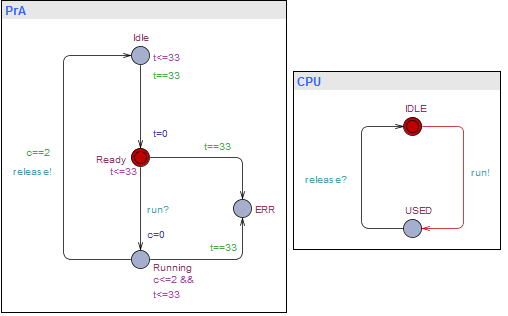
\includegraphics[scale=0.60]{billeder/UPPAALPr}}
	\caption{Automata in UPPAAL}
	\label{robot}
\end{figure}

\chapter{Tests}
\label{chap:Tests}

\section{UPPAAL schedulability analysis}
\label{sec:UPPAAL schedulability}
As described in Appendix \ref{sec:i3UPPAAL model}, Dumpsty contains three tasks: PrA, PrB and PrC. These three tasks all have individual WCET, which is not calculated, but rather tested, since calculating these through assembly proved to be impossible due to unbound loops in libraries. After testing the individual task's WCET, the worst case found would be significantly faster than what is labelled in UPPAAL, since the probability of hitting the actual worst case is close to impossible with the amount of tests done. In the following bulletpoints, all three tasks tested WCET and the WCET used in UPPAAL for the specific task is expressed, which is the first step to verify the schedulability of Dumpsty's tasks.

\begin{itemize}
	\item PrA \tab Tested: 1067 microseconds \tab UPPAAL: 2 milliseconds
	\item PrB \tab Tested: 732  microseconds \tab UPPAAL: 1 milliseconds
	\item PrC \tab	Tested: 8469 microseconds \tab UPPAAL: 9 milliseconds
\end{itemize}

For convenience, and to simplify the analysis, all tasks contain the worst case runtime of all interrupts and interrupt handlers that might occur during the execution of the task. These interrupts are generated by the motor encoders when Dumpsty is moving.

Figure \ref{UPPAAL Automata} depicts the automatas created in UPPAAL from two declared classes. The first class, task PrA, is the cyclic executive instance for the task PrA. The second class is simply a CPU which is the key needed to run the task. Every task can grab the CPU, but only one may hold it at any given time. The CPU is then released when the task is done executing, and another task can then proceed to run.

\begin{figure}[h]
	\centering
	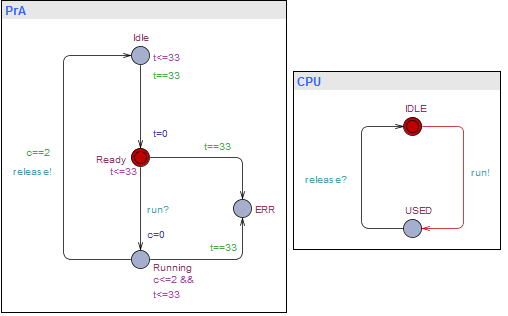
\includegraphics[scale=1]{billeder/UPPAALPr}
	\caption{Automata in UPPAAL}
	\label{UPPAAL Automata}
\end{figure}

In UPPAAL these automatas might have more than one instance, defined by the amount of tasks declared. In this case, there are three instances of the first class:

\begin{itemize}
	\item PrA = TASK(1, 33, 2);
	\item PrB = TASK(2, 33, 1);
	\item PrC = TASK(3, 33, 9);
\end{itemize}

The integers declared for every task have different meanings. These integers will be explained by the case task PrA. In task PrA, the integer 1 is the ID for the task, 33 is the deadline for the task in milliseconds, and 2 is the worst-case execution time for the task. The deadline for all tasks is the same, since this is the minimal interarrival-time(MIT) for coordinates from the Kinect sensor. All code has to be executed within the MIT of these coordinates, since a new coordinate will alter the path the robot choose.

The last step in the UPPAAL schedulability analysis is to use the verifier. This is done with two queries, found in listing \ref{Queries}. The first query checks if after some amount of time, greater than zero, all tasks has been executed at least once and all tasks are in the ready state. The second query checks that no task ever hits an error-state. If these two queries both succeed, the tasks can all be executed within the deadline, and the schedulability analysis is successful, and in this case, with tasks PrA, PrB and PrC, the tasks are schedulable within the deadlines.

\begin{lstlisting}[caption={Queries for UPPAAL}, label={Queries}]
E<> PrA.Ready and PrB.Ready and PrC.Ready and PrA.t==0 and PrB.t==0 and PrC.t==0 and time>0
E[] not (PrA.ERR or PrB.ERR or PrC.ERR)
\end{lstlisting}

\section{Unit test}
\label{sec:Unit test}
To make the unit test on the arduino code, the library ArduinoUnit has been used \citep{au}. For the arduino code there have been conducted 12 unit tests, which have been split up into two different kind of unit tests, to test the two functions driveTowardsGoal() and updatePosAndHead(). \newline
The coordinates sent to Dumpsty in the unit tests are simulated, since this is the best representation of how this robot would work under perfect conditions. These unit tests reflect how Dumpsty performs in an environment with instantaneous received data from a sensor with great precision, where the sensor will send new data every 33ms. 
The first type will test the function driveTowardsGoal() and has 3 different inputs being starting position, goal position and the heading of the robot. The robot will start at its starting position with the given heading and will then have to move towards the goal position. In the description of the test, if no heading described the heading is 0. For a code near prospective of this unit test type, check listing \ref{ut1}.

\begin{lstlisting}[caption={First type of Unit test}, label={ut1}]
test(curPos30\_150goalPos30\_150Head1){
	heading = itok(1);
	posX = itok(30);
	posY = itok(150);
	goalX = itok(30);
	goalY = itok(150);
	String result = driveTowardsGoal();
	assertEqual(result, "goal");
}
\end{lstlisting}

The second type of unit test will test the function updatePosAndHead(). The test takes 4 inputs being the starting position, the heading, millimetres to move on the right motor and millimetres to move on the left motor. The robot will start at its starting position with the given heading, and will move the given millimetres for each motor. Then the unit test will check if the robot is within 0.01mm of the asserted position.  An example of this type of unit test can been found in listing \ref{ut2}.

\begin{lstlisting}[caption={Second type of Unit test}, label={ut2}]
test(pos300_250Head075Left12Right5){
	heading = ftok(0.75);
	posX = itok(300);
	posY = itok(250);
	rightTotal = 5;
	rightTemp = 0;
	leftTotal = 12;
	leftTemp = 0;

	updatePosAndHead();

	assertMore(posX, ftok(302.826));
	assertLess(posX, ftok(302.836)); 

	assertMore(posY, ftok(253.034));
	assertLess(posY, ftok(253.044));

	assertMore(heading, ftok(0.717));
	assertLess(heading, ftok(0.727));  
}
\end{lstlisting}

Table \ref{table:Unit tests} includes all the unit tests made for the arduino code. The table consists of a description of the unit test and if the test passed or failed. 
\begin{table}
\begin{center}
	\begin{tabular}{ | p{10cm} | p{5cm} |}
		\hline
		\textbf{Test description} & \textbf{Result} \\ \hline	
		The robot is at position (30, 150), and gets the same coordinate sent, this will check if the robot says it is at goal or will try move to a new position. & Passed \\ \hline
		The robot will have a starting position at (0, 0) and will be given a new coordinate at (0, 150), the robot should then drive forward in a straight line. & \textcolor{red}{Failed} \\ \hline
		The robot will start at position (0, 0) with a heading of (1) and will be given the new coordinate (0, -150) which should make the robot turn left.  & Passed \\ \hline
		The robots starting position is (150, 150) with a heading of (-1) and is given a new coordinate at (140, 100). This means the robot will be pointing towards the top right and will have to drive down towards the right. & \textcolor{red}{Failed} \\ \hline
		The robot starts in position (150, 150) with a heading of (-1) making the robot point towards the top right. The robot is then given a new coordinate (300, 200), the robot should then turn around it self and move towards the top left & Passed \\ \hline
		The robots starting position is (0, 0) with a heading of (1), making the robot point towards the top left. The robot is given a new coordiante (0, 300). The robot will only use one motor till its heading is 0, and then drive forwards to the new coordinate  & Passed \\ \hline
		The robots starting position is (0, 0) and is given the new coordinate (-150, 300). The robot should the move towards the new position at the top right. & Passed \\ \hline
		The robot has the starting position (300, 250) with a heading of (0.75). The robot is ordered to drive 5mm with the right motor, and 12mm with the left motor and check if the new position is within a precision of 0.01mm of the asserted position. & Passed \\ \hline
		The robot has the starting position (160, 100) with a heading of (-0.4) and is to drive 14mm with the right motor and 3mm with the left motor. The robot should be within 0.01mm of the asserted position & Passed \\ \hline
		The robot is at starting position (120, 200) with a heading of (1). The robot is to drive 10mm with each motor, and be within 0.01mm of the asserted position & Passed \\ \hline
		The robot has the starting position (0, 0) and the robot is to drive 10mm with the right motor. The robot should be within 0.01mm of thte asserted position & Passed \\ \hline
		The robot has the starting position (0, 0) and the robot is to drive 10mm with the left motor. The robot should be within 0.01mm of thte asserted position & Passed \\ \hline
	\end{tabular}
	\caption{Table of conducted unit tests}
	\label{table:Unit tests}
\end{center}
\end{table}

All the failed test have been corrected and is now working as expected. 

\section{Functional test}
\label{sec:LasseSucks}
Now that the unit tests for Dumpsty are successful, the functionality of Dumpsty must be tested as well. This is done through a functional test, where Dumpsty is placed in an appropriate environment, and then the entire system will be tested. This is done through throwing a ball in front of the Kinect sensor, and having the Kinect print the sent coordinates, and having the robot moving to the point. The actual impact point of the ball will also be marked on the ground, and the distance between all three points will be measured in cm, shown in table \ref{table:FuncTest}. \newline
The three columns depicts the following:\newline
Predicted to impact: The distance from the predicted coordinate from the Kinect, to the actual impact point of the ball.\newline
Predicted to robot: The distance from the predicted coordinate to the robot, after the robot has stopped moving.\newline
Robot to impact: The distance from the robot after it has stopped moving, to the actual impact point of the ball.

\begin{table}
	\begin{center}
		\begin{tabular}{ | p{5cm} | p{5cm} | p{5cm} |}
			\hline
			\textbf{Predicted to impact} & \textbf{Predicted to robot} & \textbf{Robot to impact} \\ \hline
			23 & 11 & 34 \\ \hline
			11.5 & 6.5 & 14 \\ \hline
			19.5 & 8 & 26 \\ \hline
			19 & 10.5 & 26.5 \\ \hline
			36 & 8.5 & 43.5 \\ \hline
			48 & 11 & 56 \\ \hline
			9.5 & 11 & 21 \\ \hline
			16 & 5.5 & 11 \\ \hline
			49.5 & 11 & 48.5 \\ \hline
			13 & 11 & 19 \\ \hline
			
		\end{tabular}
		\caption{Table of conducted functional tests}
		\label{table:FuncTest}
	\end{center}
\end{table}

As one can see, Dumpsty is consistently close to 10 cm from the predicted coordinates, which could be caused by the servo motors drift after the motors has been released in the code. The fact that the prediction has a range of misprediction of 10 - 50 cm is either due to miscalculations in the Kinect code, or the Kinect having hardware issues, creating a distorted depth-picture.

%% Teknisk %%


%% Afrunding %%
\chapter{Discussion}
\label{chap:Discussion}
The discussion chapter will describe some of the choices made through the project and problems that have occurred. The problem and choices will be described and discussed, what happened and what could have been done differently. 

\subsubsection{Scheduling}
For the schedulability analysis, the WCET of the Arduino code had to be calculated. In the course, we learned that this could be done either with a language constructed timer, by counting clock cycles in the assembly code, or by using a tool. In our case, we used the tool Bound-T, without success. Our first idea was that a tool could provide WCET calculations for a piece of code, but because we were using libraries and loops which are not supported by Bound-T, it reported errors without a usable output. So our next idea was to calculate the WCET by analyzing the assembly code, but yet again the libraries proved to be a problem, since the source code of some libraries were inaccessible and contained unbounded loops. We tried counting the clock cycles, as shown in Appendix \ref{sec:i3Scheduling}. The next much coarser solution we tried was to estimate a worst-case running time for entire pieces of code, by using the timer implemented in the Arduino IDE. This is not a provable WCET estimate, since the odds of ever hitting the worst run time would be close to nonexistent in the little sample-size we provided. This lead to us almost doubling the WCET estimate in the UPPAAL model, as we already knew that the tasks were schedulable, even with a far greater WCET than what was estimated by the timer.

\subsubsection{Hardware choices}
To introduce other classical real-time concerns such as memory and execution time into this project, another platform smaller and slower than the Arduino Mega 2560 should’ve been chosen, since we only partly utilized the Arduino Mega 2560’s processor power. 

The two shields and their libraries for this project, the Arduino Motor Shield and the Arduino WiFi Shield, are helping us writing code to control the NXT servo motors and connecting to the network. When using both shields at the same time, some complications occurred. This is because the shields are using some of the same pins on the Arduino board. To work around this problem, it was decided to change the Arduino code such that it first connect to the network which will change a boolean to true and then initialize the motor shield components for use. This also means that it is not possible to continuously get new data from the Kinect, as it will send the first coordinate it captures and predicts of the thrown object. \newline

The motor shield should be used to control the motors, but an other solution to send the Kinect data to the arduino shield could be used. Either we should look for another WiFi component for the arduino, a bluetooth component or the robot should just be connected to the computer controlling the Kinect via a USB cable. 

As mentioned in chapter \ref{chap:Tests} about tests, the Kinect doesn’t reliably predict where the thrown object lands. In this project the depth sensor of the Kinect has been used, to calculate the impact point of the thrown object. Since the Kinect didn’t predict the impact point reliably, either the calculations made in the code should be revised or another way of using the Kinect should be taken into consideration. It is also possible that the Kinect didn’t function properly. 

Another important hardware issue in this project is the NXT servo motors. These motors capabilities severely limits the whole system’s capabilities. The motors set the boundaries of how far Dumpsty can move within a certain time limit paired with the circumference of the wheels. Having faster motors would also help on the response time of Dumpsty.


\subsubsection{Delimitations}
For this project we made two delimitations to the project, which can be found in section \ref{sec:Delimitations}. As mentioned, only one object will be thrown at any given time. This is an environmental delimitation, to not consider multiple objects at once. \newline
Another delimitation made was that the robot should not drive to coordinate points behind itself within the predefined area, but this is actually possible for the robot to do, also outside the predefined area. A problem we should have realized much earlier is that it is not possible for the robot to catch the object, unless it lands extremely close to the robot’s starting position, because of time spent processing, sending a signal and limitations of the motor. Another delimitations should have been made that the robot should not try to catch the object, but rather drive to the point where the object hit the ground. \newline
Instead the predefined area should not be considered and the robot should have a starting point at (0, 0), as shown in figure \ref{figure:discussion-graph} as the red dot. The robot should then be able to move to both of the blue crosses(direction of the old predefined area, but not limited to the old predefined area) and the green crosses behind the robot’s starting position. Meaning the robot only have a starting position at (0, 0), and the distance it can move on either axis is not limited, as it was with the predefined area. The robot should then drive to the predicted impact point of the object and just mark where the object had landed.


\begin{figure}[h]
	\centering
	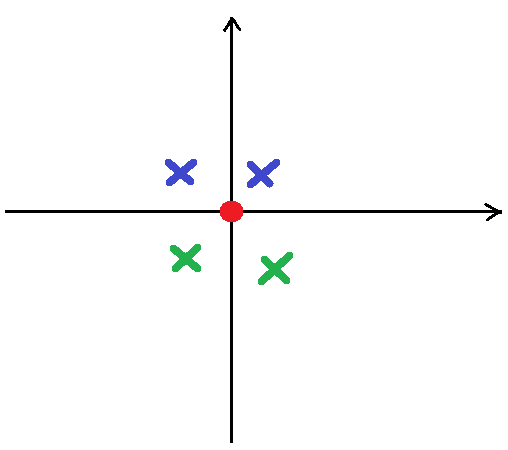
\includegraphics[scale=0.5]{billeder/discussion-graph.png}
	\caption{Graph describing the coordinate set with no predefined area}
	\label{figure:discussion-graph}
\end{figure}


\subsubsection{Process analysis}
The process model used for this project is a reflective model of the processes we have constructed our earlier projects from. This process model is based on our experience with problem based learning, and includes the processes we usually undergo through a project. It is inspired by XP, including pair programming and agile development with incrementally changing requirements. If the solution to our problem would be a safety critical solution, a more test-driven process model would be more suitable. \newline
The process model itself has worked out rather well since it isn’t restrictive and provides a very large degree of freedom when working with the project, compared to a rigid adherence to a well established model, such as the waterfall model. \newline
After experimenting with the process model throughout this project it has come to our attention that some changes should be made to the structure of the process model. A more explicit test section should be implemented to test all interdependent components, and ensure that all increments’ implementations work as intended. This will in turn also increase the coherence between each increment. This test section will also include tests across each increment, to check that no new errors has been introduced to earlier implementation.





\chapter{Conclusion}
\label{chap:Conclusion}
Based on chapter \ref{chap:Analysis} concerning a user story, system capabilities, hardware's capabilities and limitations, lead to the project’s problem statement: 


\textbf{\textit{How can an embedded system control a trash bin to detect, track and catch a thrown object within a designated area?}}


The final system partially solves the problem statement. It is capable of detecting and tracking the object thrown towards the robot, but not consistently catch it, because of the hardware limitations for the project, these limitations are mentioned in the discussion \ref{chap:Discussion}. 


To solve the problem statement, a list of general requirements with related sub requirements were constructed. In the following paragraphs each of the general requirements will be evaluated. 


\subsubsection{The trash bin should catch the object if the user throws it towards the trash bin and within a predefined area}
\label{sub:1}
This requirement was not accomplished, since the robot was not reliably able to move to the impact point of the thrown object. No trash bin has been attached on top of the robot, which would determine the area in which it is able to catch the object, but it is still considerably inaccurate by 10-50 cm from the actual impact point to the robot’s final position. If the estimated coordinate sent by the Kinect was true, it would consistently be 11 cm inaccurate, because of the robot drifting past the point after releasing the motors. \newline
We ended up not taking the predefined area into account, it was used in the design phase to measure where the robot would be able to catch a thrown object, but it was not useable because its movement was too slow and the time used in data transfer compared to object flight time was a greater obstacle than expected. Thus it was not useful in the final product.




\subsubsection{The robot should know where it is positioned}
This requirement is fulfilled. The robot has variables of its current position as an X and Y coordinate set and its heading. These values are updated in the Arduino loop function using the encoders of the motors. When the robot reaches its destination the robot shuts down, but the servo motors drift, usually 11 cm, which is not considered to the current position of the robot. This would accumulate if the robot is not reset, and placed on the position (0, 0) after every run.


\subsubsection{The robot should be able to detect and track the thrown object}
As the Kinect is used as a sensor for the robot, this requirement is fulfilled. The reason is because the Kinect is able to both detect and track the object. It is not able to detect every object thrown, and some times it detects other objects such as a human limb or something in the distortion in the room. \newline
When the first impact point of the thrown object has been sent from the Kinect, it will keep tracking the object, but the robot will not receive further data, therefore the robot is not continuously tracking the object after the first impact point is received.  


\subsubsection{The robot should be able to calculate the impact point for the object}
The Kinect sends the predicted impact point of the object to the robot. This impact point is not accurate, as mentioned before the robot is stopping 10-50 cm away from the predicted impact point. We would say that this requirement is partially fulfilled, because it can calculate an impact point, but not a precise impact point. This requirements success is scaled from how big of a bin is placed on top of the robot, and the size of the thrown object.


\subsubsection{The robot should be able to move the trash bin, such that the thrown trash lands inside the bin} 
No trash bin has been attached to the robot, so this requirement is not fulfilled. If a trash bin had been attached to the robot, it should have a radius greater than 11 cm to catch the object, since 11 cm was the closest the robot was to the impact point.


\subsubsection{The robot should be able to receive data from a computer, through a wireless network} This requirement is fulfilled. The computer connected to the Kinect is able to send the recorded data to the robot. 


\subsubsection{The system tasks should be able to be scheduled and verified}
This requirement is fulfilled by the UPPAAL schedulability analysis as described in section \ref{sec:UPPAAL schedulability} in the test chapter.


\subsubsection{Conclusion}
When considering the success of this project, the final product is somewhat a success. One can conclude that the hardware does not meet the time constraints of the problem, and the prediction is not reliable. When a user throws an object towards the robot, it is not able to catch the object, but it is able to give a prediction of the impact point, it is able to move the robot to the coordinates of the prediction, but will drift past the coordinates. The robot is able to position itself accordingly to the starting point, but it will not be able to continuously position itself after stopping at the impact point. The drift makes the robot unable to position correctly, so the robot has to be repositioned to the correct starting point after each use.\newline


The robot is able to receive data from the Kinect sensor through a wireless network, and all the tasks for the system are schedulable, and the fact that this embedded system provides a basis for a solution to the problem concludes this as a successful system in our opinion.
The biggest objective in this project was to learn about embedded systems and real time problems. Although this project did not concern many of the classical embedded systems problems, a cyclic executive was constructed and the analysis involved. Although considerations of memory management and cpu speed was not present, some considerations were performed. Even when considering the initial preconceived notions of the platform, motors and Kinect alot of unexpected problems arose, some of which were solved and others would need different hardware to solve the problem statement.  

\include{formalia/futurework}

%%%% Kilder %%%%

\begingroup
	\raggedright
	\bibliography{bibtex/litteratur}							% Litteraturlisten inkluderes
\endgroup


%%%% Fixme-listen %%%%

\newpage														% Ny side til Fixme-listen
%\listoffixmes													% Fixme-listen - fjernes til sidst i projektet med "%"


%%%% Appendiks %%%%

\appendix														% Appendiks/bilag start - giver chapter bogstaver i stedet for tal
\clearforchapter												% Sikrer at pagestylen aktiveres paa den rigtige side
\phantomsection													% Kunstigt afsnit, som hyperlinks kan 'holde fast i'
\pdfbookmark[0]{Appendiks}{appendiks}							% Tildeler en klikbar bookmark til den endelige PDF

%% Indstillinger for appendiks (deaktiveret med "%") %%

%\pagestyle{empty}												% Sidehoved/-fod for standardsider aendres til tom for appendiks
%\aliaspagestyle{chapter}{empty}								% Sidehoved/-fod for kapitelsider aendres til tom for appendiks
%\settocdepth{chapter}											% Kun kapitel-niveau vises i ToC
%\addtocontents{toc}{\protect\cftpagenumbersoff{chapter}}		% Sidetal for kapitler fjernes i ToC

%% Filer til appendiks %%

\chapter{Appendix}
\label{chap:Appendix}


%%%% Bilag %%%%

%\phantomsection												% Kunstigt afsnit, som hyperlinks kan 'holde fast i'
%\addcontentsline{toc}{chapter}{Bilag A \ Navn} 				% Manuelle indgange i indholdsfortegnelsen (naar \includepdf bruges)

%\includepdf[pages={x-y}]{filnavn}								% Inkluder eksterne bilag med \includepdf[pages={x-y}]{filnavn}


\end{document}													% Slutter dokumentet - obligatorisk


